\documentclass[a4paper, fleqn, 9pt]{extarticle}
\usepackage{etoolbox}
\usepackage{Alegreya, euler}

\usepackage{amssymb, mathrsfs}
\usepackage[left=1.5cm,top=2.5cm,right=1.5cm,bottom=1.5cm]{geometry}
\usepackage{multicol}
\usepackage{MnSymbol}

\usepackage{fancyhdr}
\makeatletter
\fancypagestyle{mypagestyle}
{\newpage \fancyfoot[C]{} \renewcommand{\footrulewidth}{0pt}}
\makeatother
\pagestyle{mypagestyle}
\headsep 5pt                 %% put this outside
\usepackage{lastpage}

\usepackage[usenames,dvipsnames]{color}
\usepackage{xcolor}

\newcommand{\prawo}[1]{\marginpar{\textbf{\underline{#1}}}}
\newcommand{\wcht}[1]{{\bf {#1}}}
\newcommand{\spk}{\, \bullet \,}
\newcommand{\datum}[1]{{\color{Purple} \bf {#1}}}

% ? - pożyteczne zbiory
\newcommand{\K}{\mathbb{K}}
\newcommand{\C}{\mathbb{C}}
\newcommand{\N}{\mathbb{N}}
\newcommand{\R}{\mathbb{R}}
\newcommand{\Q}{\mathbb{Q}}
\newcommand{\Z}{\mathbb{Z}}
\newcommand{\Qp}{\mathbb{Q}_p}
\newcommand{\Zp}{\mathbb{Z}_p}

% Logika
\newcommand{\Lra}{\Leftrightarrow}
\newcommand{\Ra}{\Rightarrow}

% Algebra
\newcommand{\trk}{\trianglelefteq}
\newcommand{\im}{\operatorname{im}}
\newcommand{\autgrp}{\operatorname{Aut}}
\newcommand{\inngrp}{\operatorname{Inn}}
\newcommand{\outgrp}{\operatorname{Out}}
\newcommand{\holmrf}{\operatorname{Hol}}























% Analiza
%\newcommand{\D}{\textrm{d}}
%\DeclareMathOperator{\grad}{grad}
%\DeclareMathOperator{\rot}{rot}
%\DeclareMathOperator{\dvrg}{div}

% Miara
%\newcommand{\Rr}{\overline \R}

% Algebra abstrakcyjna

%\newcommand{\krt}{\trianglerighteq}


% Topologia
%\DeclareMathOperator{\cl}{cl}
%\DeclareMathOperator{\interior}{int}

% Pstwo
%\DeclareMathOperator{\pstwo}{\mathcal{P}}
%\DeclareMathOperator{\esssup}{ess\,sup}
%\newcommand{\expected}{\mathbb{E}}
%\newcommand{\variance}{\mathbb{V}}
%\newcommand{\prawie}{\leadsto}
%\newcommand{\wgpstwa}{\rightarrowtail}
%\newcommand{\wgrozkladu}{\twoheadrightarrow}

% Liniowa
%\newcommand{\rank}{\operatorname{rank}}
%\newcommand{\chara}{\operatorname{char}}
%\newcommand{\pf}{\operatorname{Pf}}
%\newcommand{\ann}{\operatorname{Ann}}

% \DeclareMathOperator{\autom}{\mathcal A}
% \DeclareMathOperator{\centror}{\mathcal C}
% \DeclareMathOperator{\chara}{char}
% \DeclareMathOperator{\cl}{cl}
% \DeclareMathOperator{\covariance}{cov}
% \DeclareMathOperator{\diam}{diam}
% \DeclareMathOperator{\disexp}{Exp}
% \DeclareMathOperator{\esssup}{ess\,sup}
% \DeclareMathOperator{\grupapsl}{\mathrm{PSL}}
% \DeclareMathOperator{\holomorf}{\mathcal H}
% \DeclareMathOperator{\innerm}{\mathcal I}
% \DeclareMathOperator{\interior}{int}
% \DeclareMathOperator{\normor}{\mathcal N}
% \DeclareMathOperator{\outerm}{\mathcal O}
% \DeclareMathOperator{\rad}{rad}
% \DeclareMathOperator{\rot}{rot}
% \DeclareMathOperator{\zenter}{\mathcal Z}
% \newcommand{\Ab}{\catname{Ab}}
% \newcommand{\Aut}{{\textrm {Aut}}}
% \newcommand{\bigslant}[2]{{\raisebox{.2em}{$#1$}\left/\raisebox{-.2em}{$#2$}\right.}}
% \newcommand{\calka}[4] {\int_{\farbea{#1}}^{\farbeb{#2}} #3 \, \textrm{d}{#4}}
% \newcommand{\catname}[1]{{\normalfont\textbf{#1}}}
% \newcommand{\cf}{\text{cf }}
% \newcommand{\Ci}{\operatorname{Ci}}
% \newcommand{\col}{\mathit{Col}}
% \newcommand{\cov}{\text{cov }}
% \newcommand{\Cp}{\mathbb{C}_p}
% \newcommand{\CRng}{\catname{CRng}}
% \newcommand{\dotr}[1]{#1^{\cdot}} 
% \newcommand{\dvrg}{\textrm{div }}
% \newcommand{\dwumk}[2] {\left[{#1 \atop #2}\right]}
% \newcommand{\dwumo}[2] {\left\{{#1 \atop #2}\right\}}
% \newcommand{\dwump}[2] {\left\{\begin{matrix} #1\\ #2\\ \end{matrix} \right\}}
% \newcommand{\dwum}[2] {\left({#1 \atop #2}\right)}
% \newcommand{\Ei}{\operatorname{Ei}}
% \newcommand{\ex}{{\textrm E}}
% \newcommand{\Fp}{\mathbb{F}_p}
% \newcommand{\grad}{\text{grad }}
% \newcommand{\Grp}{\catname{Grp}}
% \newcommand{\hipergeo}[3] {\left(\left.{#1 \atope #2}\,\right|\,#3\right)}
% \newcommand{\igr}{{\textrm Y}}
% \newcommand{\iks}{{\textrm X}}
% \newcommand{\imaz}{\mathfrak{Im } }
% \newcommand{\imp}{\bf}
% \newcommand{\inj}{\hookrightarrow}
% \newcommand{\kalendarz}{\color{wordblu} \bf}
% \newcommand{\kcod}{\textrm{cod }}
% \newcommand{\kdom}{\textrm{dom }}
% \newcommand{\khom}{\textrm{hom}}
% \newcommand{\kid}[1]{\textrm{id}_{#1} }
% \newcommand{\kkcod}{\textrm{cod }}
% \newcommand{\kkdom}{\textrm{dom }}
% \newcommand{\kkid}[1]{\textrm{id}_{#1} }
% \newcommand{\krt}{\trianglerighteq}
% \newcommand{\K}{\mathbb{K}}
% \newcommand{\li}{\operatorname{li}}
% \newcommand{\lk}{\mathit{lk}}
% \newcommand{\mydelta}{{\color{wordred}\delta}}
% \newcommand{\mysigma}{{\color{wordred}\sigma}}
% \newcommand{\oprot}{\text{rot }}
% \newcommand{\pf}{\text{Pf }}
% \newcommand{\pocho}[2] {{#1}^{\overline{#2}}}
% \newcommand{\pochu}[2] {{#1}^{\underline{#2}}}
% \newcommand{\PSL}{\text{PSL}}
% \newcommand{\rank}{\text{rank }}
% \newcommand{\reel}{\mathfrak{Re }\, }
% \newcommand{\rhn}[1] {\left \lsem {#1} \right \rsem}
% \newcommand{\Span}{\mathit{span}}
% \newcommand{\sqrr}[1] {#1^{1/2}}
% \newcommand{\stda}{\color{wordblu}}
% \newcommand{\stdb}{\color{wordblu}}
% \newcommand{\summ}{\sum_{m=1}^\infty}
% \newcommand{\sumn}{\sum_{n=1}^\infty}
% \newcommand{\surj}{\twoheadrightarrow}
% \newcommand{\Top}{\catname{Top}}
% \newcommand{\tostar}{\ensuremath{\mathaccent\star\to}}
% \newcommand{\unif}{\rightrightarrows}

\usepackage{graphicx}
\relpenalty=10000
\binoppenalty=10000
\interlinepenalty=10000

\newenvironment{enumx}{\begin{enumerate} \setlength{\itemsep}{0pt} \setlength{\parskip}{0pt} \setlength{\parsep}{0pt}}{\end{enumerate}}
\newenvironment{itemx}{\begin{itemize} \setlength{\itemsep}{0pt} \setlength{\parskip}{0pt} \setlength{\parsep}{0pt}}{\end{itemize}}


\usepackage[polish]{babel}
\usepackage[utf8]{inputenc}
\usepackage[T1]{fontenc}
\selectlanguage{polish}

\begin{document}
\setlength{\belowdisplayskip}{2pt}
\setlength{\belowdisplayshortskip}{2pt}
\setlength{\abovedisplayskip}{2pt}
\setlength{\abovedisplayshortskip}{2pt}


\renewcommand{\footrulewidth}{0.4pt}
\fancyhead[LE,LO]{Zwyczajne równania różniczkowe (MSC 34)}
\fancyhead[RO,RE]{leon.aragones@gmail.com, listopad 2015}
\fancyfoot[RF]{w przypadku równań nieczosnkowych, $y$ jest funkcją $x$}


\begin{multicols*}{2}
\begin{enumx}
\item \textbf{Równanie Airy'ego/Stokesa}: $y'' - xy = 0$ z rozwiązaniem danym przez szereg $\sum_{n \ge 0} a_n x^n$.
Ma nz rozwiązania $y_i$ albo jako funkcje Airy'ego.
\begin{align*}
 y_1(x) & = a_0 \left[1 + \sum_{n=1}^\infty \frac{(3n-2)!!!}{(3n)!} \cdot x^{3n} \right] \\
 y_2(x) & = a_1 \left[x + \sum_{n=1}^\infty \frac{(3n-1)!!!}{(3n+1)!} \cdot x^{3n+1}\right] \\
 Ai(x) & = \frac 1 \pi \int_0^\infty \cos (xt + t^3:3) \, \D t \\
 Bi(x) & = \frac 1 \pi \int_0^\infty [\exp (x t - t^3:3) + \sin (xt + t^3:3)] \,\D t
\end{align*}
\end{enumx}
\begin{center}
	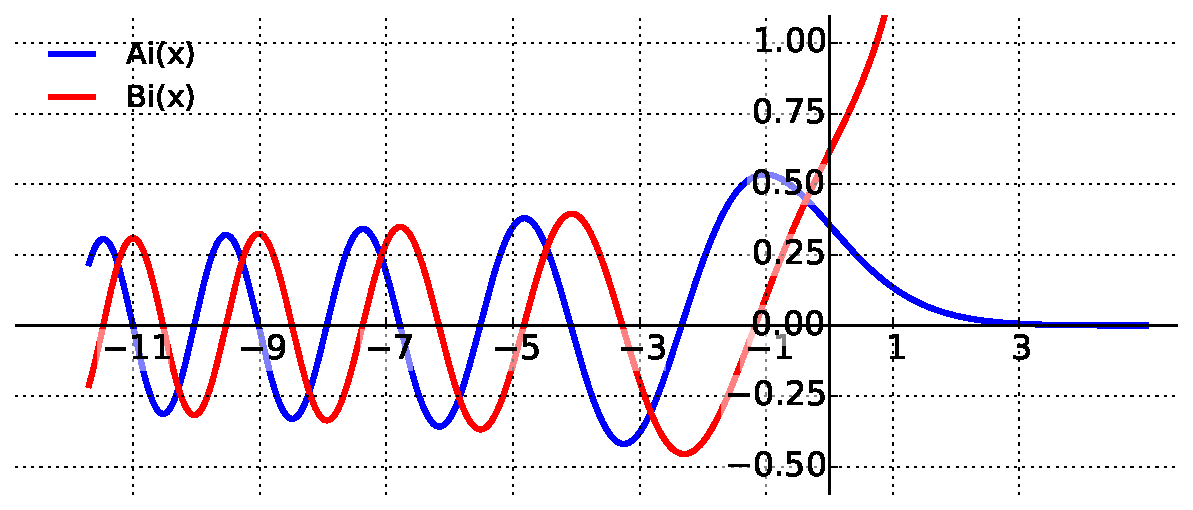
\includegraphics[width=0.9\columnwidth]{airy.pdf}
\end{center}
\begin{enumx}
\item \textbf{Równanie Airy'ego}, uogólnione: $y''' - 4xy'- 2y = 0$.
Rozwiązaniami są: $\operatorname{Ai}^2$,  $\operatorname{Ai} \operatorname{Bi}$ oraz $\operatorname{Bi}^2$.
%\item \textbf{Równanie d'Alemberta}: $y = \varphi(y') + \psi(y')$.
%Niech $p = y'$, wtedy mamy $p - \varphi(p) = [x \varphi'(p) + \psi'(p)] p'(x)$.
%Mamy też $y=rx + \psi(r)$, gdzie $r$ zeruje lewą stronę (specjalne).
%Kiedy ich nie ma, jest problem.
\item \textbf{Równanie Bernoulliego}: $y' + f y = g y^k$.
Trzeba je podzielić przez $y^k$ i podstawić $z = y^{1 - k}$.
\item \textbf{Równanie Bessela}: $x^2 y'' + xy' + (x^2 - p^2) y = 0$.
Próbujemy szeregu: $y = \sum_{m \ge 0} a_m x^{r+m}$ z $a_0 \neq 0$.
Wtedy $a_0(r^2 - p^2) = a_1 [(r+1)^2 - p^2] = 0$, dla $m \ge 2$: $a_{m-2} = a_m[p^2 - (r+m)^2]$.
Jeżeli $r = p$, rozwiązaniem jest funkcja Bessela rzędu $p$, $J_p$.
Jeżeli $p \not \in \Z$, to $J_p$ oraz $J_{-p}$ są niezależne.
Jeżeli $p \in \Z$, trzeba użyć funkcji Bessela drugiego rodzaju, $Y_p$.
\begin{align*}
J_p(x) & = \sum_{k \ge 0} \frac{(-1)^k (x : 2)^{2k+p}}{k! \cdot \Gamma(k + p + 1)} \\
Y_p(x) & = \lim_{v \to p} [J_p(x) \cos p \pi - J_{-p}(x)] : (\sin p \pi)
\end{align*}
\end{enumx}
\begin{center}
	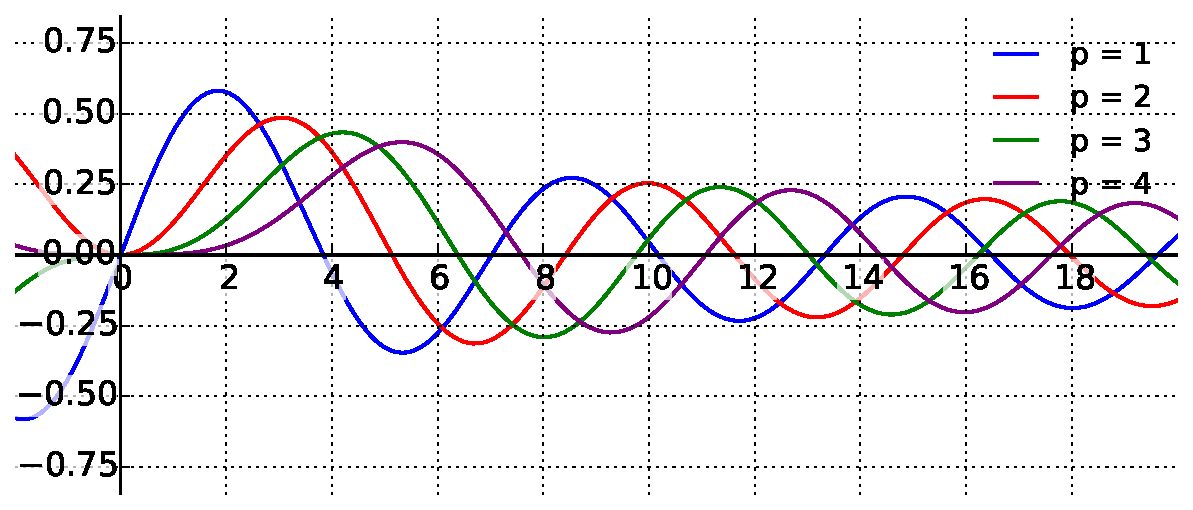
\includegraphics[width=0.9\columnwidth]{bessel.pdf}
\end{center}
\begin{enumx}
\item \textbf{Równanie Clairauta}: $y = xy' + \psi(y')$.
Niech $p = y'$. Zróżniczkowanie daje $[x + \psi'(p)] p'(x) = 0$, a w $\R$ nie ma dzielników zera.
\item \textbf{Równanie Eulera}: $x^2 y'' + axy' + by = 0$. Rozwiązania: dla $(1-a)^2 > 4b$ ($y_1$), dla $(1-a)^2 = 4b$ ($y_2$) i $(1-a)^2 < 4b$ ($y_3$); $2 \mu = |(1-a)^2 - 4b|^{1:2}$.
\begin{align*}
y_1(x) & = |x|^{(1-a):2} (A |x|^\mu + B |x|^{- \mu}) \\
y_2(x) & = |x|^{(1-a):2} (A + B  \ln |x|) \\
y_3(x) & = |x|^{(1-a):2} (A \sin (\mu \ln |x|) + B \cos (\mu \ln |x|)) 
\end{align*}
\item \textbf{Równanie Hermite'a}: $y'' - 2 x y' + 2 ny = 0$ dla $n \in \R$.
Jeżeli $y_i$ są jak niżej, to $Af_1 + Bf_2$ jest ogólnym rozwiązaniem ($A, B \in \R$).
\begin{align*}
y_1(x) & = \sum_{k=0}^\infty \frac{2^k x^{2k+1}}{(2k+1)!} \prod_{t=0}^{k-1} (2t+1-n)  \\
y_2(x) & = \sum_{k=0}^\infty \frac{2^k x^{2k}}{(2k)!} \prod_{t=0}^{k-1} (2t-n)
\end{align*}
\item \textbf{Legendre'a}: $(1-x^2)y'' - 2xy' + n(n+1) y = 0$.
Rozwiązania dane są przez $A P_n(x) + BQ_n(x)$, gdzie
\begin{align*}
P_n(x) & = \frac{d^n}{n! 2^n dx^n} (x^2-1)^n\\
Q_n(x) & = \frac 12 P_n(x) \ln \frac{1+x}{1-x} - \sum_{m =1}^n \frac 1 m P_{m-1}(x) P_{n-m}(x)
\end{align*}
\item \textbf{Równanie Riccatiego}: $y' = f + g y + h y^2$.
Podstawienie $y = - w' : [h w ]$ coś może uprościć.
Jeśli znamy rozwiązanie $y_0(x)$, to $y := y_0 + 1 : w$
przekształca równanie do $w' + [g + 2h y_0] w + h = 0$.
\item \textbf{Równanie van der Pola}: $y'' - \mu(1 - y^2) y' + y = 0$.
Rozwiązaniami dla $\mu = 0$ są $y_0 \cos x + \dot y_0 \sin x$.
Jeżeli $\mu > 0$, to układ ma jednoznaczny cykl graniczny (przyciągający).
\item \textbf{Równanie Emdena-Fowlera}: $y'' = Ax^n y^m$.
Rozwiązanie (dla $m \neq 1$) $y = \lambda x^{(n+2):(1-m)}$ jest specjalne.
Przez $z = x^{n+2} y^{m-1}$ oraz $w = xy'/y$ dostajemy równanie Abela.
Znane rozwiązania dla:
\begin{enumx}
\item dowolnego $m$ i $n = 0, -m-3$ lub $-(m+3):2$.
\item dowolnego $n$ i $m = 0, 1$.
\item szczególnych przypadków:
\begin{enumx}
\item $m = -7$, $n = 1, 3$
\item $m = -5:2$, $n = -1:2$
\item $m = -2$, $n = -2, 1$
\item $m = - 5:3$, $n = -10:3, -7:3, -5:6, -1:2, 1, 2$
\item $m = -7:5$, $n = -13:5, n = 1$
\item $m = -1:2$, $n = -7:2, -5:2, -2, -4:3, -7:6, -1:2, 1$
\item $m = 2$, $n = -5, -20:7, -15:7$.
\end{enumx}
\end{enumx}
\end{enumx}

\raggedright

\begin{enumx}
\item Równania liniowe
	\begin{enumx}
	\item Laplace'a: $\Delta u = \sum_{i \le n} u_{x_ix_i} = 0$
	\item Helmholtza: $-\Delta u = \lambda u$
	\item transportu: $u_t + \sum_{i \le n} b^i u_{x_i} = 0$
	\item Liouville'a: $u_t - \sum_{i \le n} (b^i u)_{x_i} = 0$
	\item przewodnictwa cieplnego / dyfuzji: $u_t - \Delta u = 0$
	\item Schrödingera: $\textrm{i} u_t + \Delta u = 0$
	\item Kołmogorowa: $u_t - \sum_{i, j \le n} a^{ij} u_{x_ix_j} + \sum_{i \le n} b^i u_{x_i} = 0$
	\item Fokkera-Plancka: $u_t - \sum_{i, j \le n} (a^{ij} u)_{x_ix_j} + \sum_{i \le n} (b^i u)_{x_i} = 0$
	\item falowe: $u_{tt} - \Delta u = 0$
	\item telegrafistów: $u_{tt} + du_t - u_{xx} = 0$
	\item ogólne falowe: $u_{tt} + \sum_{i, j \le n} a^{ij} u_{x_ix_j} + \sum_{i \le n} b^i u_{x_i} = 0$
	\item Airy'ego: $u_t + u_{xxx} = 0$
	\item belki: $u_{tt} + u_{xxxx} = 0$
	\end{enumx}
\item Równania nieliniowe
	\begin{enumx}
	\item eikonału: $|Du| = 1$
	\item Poissona: $- \Delta u = f(u)$
	\item $p$-harmoniczne: $\operatorname{div} (|Du|^{p-2} Du) = 0$
	\item powierzchni minimalnych: $\operatorname{div} (Du (1+|Du|^2)^{-1:2})=0$
	\item Monge'a-Ampere'a: $\det D^2 u = f$
	\item Hamiltona-Jacobiego: $u_t + H(Du, x) = 0$.
	\item skalarne zachowania: $u_t + \operatorname{div} F(u)=0$
	\item Burgersa bez lepkości: $u_t + uu_x = 0$
	\item skalarne reakcji-dyfuzji: $u_t - \Delta u = f(u)$
	\item ośrodków porowatych: $u_t - \Delta (u^\gamma) = 0$
	\item falowe: $u_{tt} - \Delta u = f(u)$, $u_{tt} - \operatorname{div} a (Du) = 0$
	\item Kortewega-de Vriesa: $u_t + uu_x + u_{xxx}=0$
	\end{enumx}
\item Układy liniowe
\begin{enumx}
	\item równowagi w liniowej teorii sprężystości: $\mu \Delta u + (\lambda + \mu) D(\operatorname{div} u) = 0$
	\item ewolucyjne w liniowej teorii sprężystości: $u_{tt} - \mu \Delta u - (\lambda+\mu) D(\operatorname{div} u) = 0$
	\item Maxwella: $E_t = \operatorname{rot} B$, $B_t = - \operatorname{rot} E$, $\operatorname{div} B = \operatorname{div} E = 0$.
	\end{enumx}
\item Układy nieliniowe
\begin{enumx}
	\item praw zachowania: $u_t + \operatorname{div} F(u) = 0$
	\item reakcji-dyfuzji: $u_t - \Delta u = f(u)$
	\item Eulera nielepkiego przepływu nieściśliwego: $\operatorname{div} u = 0$, $u_t + u \cdot D u = - Dp$.
	\item Naviera-Stokesa lepkiego przepływu nieściśliwego: $\operatorname{div} u = 0$, $u_t + u \cdot D u - \Delta u = - Dp$.
	\end{enumx}
\end{enumx}

\end{multicols*}
\end{document} 

\begin{multicols}{2}
R--e rzędu dwa: $y'' = f(t,y,y')$, jeśli $y'' + p(t) y' + q(t) y = g(t)$, to liniowe, jednorodne dla $g(t) \equiv 0$.
Jeśli $p, q$ są ciągłe na przedziale, to rozwiązanie jest jedyne.
\emph{Jeśli $y_1, y_2$ są rozwiązaniami i $y_1y_2'-y_1'y_2$ nie jest zerem, to $y = c_1y_1 + c_2y_2$ jest ogólnym rozwiązaniem.}
%\zutun{WROŃSKIAN}

% Równanie niejednorodne, jak.
% Metoda wariacji parametrów
% Zgadywanie.
% Wielomian - wielomian.

\begin{enumx}
\item \textbf{Równanie $\color{blue}y'' = f(x)$} ze stałymi współczynnikami, gdzie $f$ jest ciągłą funkcją.
Dwa razy scałkować.
Z warunkami $y(x_0) = y_0$ oraz $y'(x_0) = y_0'$:
$$
	y(x) = y_0 + y_0(x-x_0) + \int_{x_0}^x f(x)(x-t) \,\textrm{d}x
$$
% \item \textbf{Rozdzielone zmienne}.
% Jednorodne: $F(x,y) \,\textrm{d}x + G(x,y)  \,\textrm{d}y = 0$, gdzie $F, G$ są jednorodne tego samego stopnia.
% Wtedy $y'(x) = -F(x,y) / G(x,y)$ zależy tylko od $y/x$, czyli $y'(x) = f(y/x)$.
% Pomocne jest $t:= y/x$, $y'(x) = t+x t'(x)$; wtedy $t + x t'(x) = f(t)$, zatem każdy pierwiastek $f(t) = t$ daje singularne rozwiązanie. Ogólne niżej w postaci parametrycznej.
% \[
% 	x = C \exp \left[ \int \frac{\textrm{d}t}{f(t)-t}\right] \,\bullet\,
% 	y = C t \exp \left[ \int \frac{\textrm{d}t}{f(t)-t}\right]
% \]
\item \textbf{Pierwszego rzędu, liniowe}: $\color{blue}y' + P(x) y = Q(x)$ dla ciągłych $P, Q$.
Czynnikiem całkującym jest tu ,,$E =  \exp(\int P(x) \,\textrm{d}x)$''.
$$
y= \left[C + \int Q(x) E(?) \,\textrm{d} x\right] \cdot \frac 1 E
$$
\item \textbf{Drugiego rzędu, liniowe, stałe współczynniki}: $\color{blue}x'' + bx' + cx = 0$, gdzie $b, c \in \mathbb R$.
%Gdy $c \neq 0$, to $(0, 0)$ jest: źródłem $\Leftrightarrow$ $b < 0$, $c > 0$; spiralnym źródłem $\Leftrightarrow$  jest źródłem i $\Delta < 0$; zlewem $\Leftrightarrow$ $b, c > 0$, spiralnym zlewem $\Leftrightarrow$ jest zlewem i $\Delta < 0$; siodłem $\Leftrightarrow$ $c < 0$; centrum $\Leftrightarrow$ $b = 0$ i $c > 0$.
Jeżeli $x(t) = e^{rt}$, to $r^2 + br + c = 0$.
Wtedy $e^{r_1t}$ i $e^{r_2t}$ ($\Delta>0$),  $e^{rt}$ i $t e^{rt}$ ($\Delta = 0$), lub (dla $r = \alpha \pm \beta i$) $e^{\alpha t}\cos (\beta t)$ oraz $e^{\alpha t} \sin (\beta t)$ to rozwiązania.
%\textbf{General solution of linear differential equation}
%Liniowe, jednorodne $\sum_{v=0}^n k_v(x)y^{(n-v)}(x) = 0$; jeśli $k_v(x)$ są ciągłe, zaś $k_0(x)$ nie znika na odcinku, to wszystkie rozwiążania są ciągłe; jeśli współczynniki mają ciągłe pochodne, to rozwiązanie też.
%Jeśli $k_0(x)$ znika w $x_0$, to jest on singularny
\item \textbf{R--e Abela}: $\color{blue}y\dot y = f(x) y^2 + g(x)y + h(x)$.
Zmienia $y = E(x) w$ je w $w \dot w = F_1(x) w + F_0(x)$.
Dalsza redukcja: $z = \int F_1\,\textrm{d}x$, $w(z)w'(z) - w(z)= \Phi(z)$, gdzie $\Phi(z)$ jest $x$-parametryczna: $\Phi = F_0(x) / F_1(x)$.
$$
	E(x) = \exp\left[\int f(x)\,\textrm{d}x\right] \spk
	F_1 = \frac g E \spk
	F_0 = \frac h{E^2}
$$
\item \textbf{R--e Airy'ego}: $\ddot y \pm k^2 xy = 0$ lub $\ddot y - xy = 0$.
Gdy $y = \sum_n a_n x^n$, to $(n+2)(n+1) a_{n+2} = a_{n-1}$ i $a_2 = 0$.
Rozwiązaniem dla r--a $\dddot{y} = 4x\dot y + 2y$ są $\textrm{Ai}(x)\textrm{Ai}(x)$, $\textrm{Ai}(x) \textrm{Bi} (x)$, $\textrm{Bi}(x)\textrm{Bi}(x)$.
\[
	y = \sum_{n=0}^\infty \left[ \frac{ a_0 x^{3n}}{\prod_{k=1}^n {3k(3k-1)}} + \frac{a_1 x^{3n+1} }{\prod_{k=1}^n {3k(3k+1)}}  \right]
\]
\[
	\textrm{Ai}(x) = \frac 1 \pi \int_0^\infty {\cos(t^3/3+xt)} \,\textrm{d}t
\]
\[
	\textrm{Bi}(x) = \frac 1 \pi \int_0^\infty {\sin(t^3/3+xt) + \exp(-t^3+xt)} \,\textrm{d}t
\]
\item \textbf{R--e d'Alemberta}: $\color{blue}y = x \phi(y') + \psi(y')$.
Gdy $p = y'$, to $p - \phi(p)$ $=$  $ [x \phi'(p) + \psi'(p)] p'$. 
Dla pierwiastków $p_1, \dots, p_k$ równania $p = \phi(p)$ są rozwiązania $y = p_v x + \psi(p_v)$.
Jeżeli $\phi(p) \not \equiv p$, to piszemy tak, jak niżej.
Dla rozwiązania $x = x(p, C)$ musi być $y = \phi(p) x(p,C) + \psi(p)$ (gdzie $C$ stałą całkowania). % (krzywe całkowe?).
 \[
	\frac{\textrm{d}x}{\textrm{d}p} = \frac{\phi'(p)}{p - \phi(p)} x + \frac{\psi'(p)}{p-\phi(p)}
	\]
\item \textbf{R--e Bernoulliego}: $\color{blue}y' + f(x) y = g(x) y^k$ ($k \neq 0, 1$). 
Dzielić przez $y^k$, podstawić $z = y^{1-k}$: $z' + (1-k)f(x) z = (1-k)g(x)$ jest wynikiem.
Opisuje ruch z oporem $F = \lambda_2 v^k + \lambda_1 v$ ($f, g$ ciągłe).
\item \textbf{R--e Bessela}: $\color{blue}x^2 y''(x) + x y'(x) + (x^2-p^2)y = 0$ z $p \ge 0$.
\[
y = x^r \sum_{k=0}^\infty a_k x^k \Ra a_{k-2} + [(r+k)^2-p^2] a_k = 0
\]
($a_k = 0$ dla $k < 0$).
Z $a_0 \neq 0$ wynika $r = \pm p$.
Jeśli $r = p$, to khm-1; w podobny sposób można odtworzyć wszystkie $a_k$: $a_{2l+1} = 0$, parzyste niżej.
Kiedy $p$ nie jest całkowite (półcałkowite), można dostać drugie rozwiązanie przez napisanie $-p$ zamiast $p$.
Gdy $p \in \mathbb N$, to $J_{-n} = (-1)^n J_n$; wtedy rozwiązań trzeba szukać w kombinacjach $J_n(x)$ i $J_n(x) \ln x + \sum_{k=0}^\infty b_k x^{k-n}$.
\begin{align*}
	a_k & = \frac{-a_{k-2}}{k(2p+k)} \Ra
	a_{2k} = \frac{(-1/4)^ka_0}{k! \cdot (p+1) \cdot \ldots \cdot (p+k)} \\ 
	y & = a_0x^{\pm p} \left[\sum_{k=1}^\infty \frac{a_{2k}x^{2k}}{a_0}\right] \quad ???
\end{align*}
\item \textbf{R--e Clairauta}: $\color{blue} y = x y' + \psi (y')$.
Zróżniczkowanie daje tu $[x + \psi'(y)] y'' = 0$, czyli $y'' = 0$ (to jest rodzina prostych) lub $x + \psi'(y') = 0$ (trudne -- gdy znajdzie się zależność $p$ od $x$, to $y = xp(x) + \psi(p(x))$ jest singularnym rozwiązaniem).
\item \textbf{R--e Czebyszewa}: $\color{blue}(1-x^2) y'' - xy' + p^2y=0$, gdzie $p \in \mathbb R$.
Dwa nz rozwiązania-szeregi  są dla $(a_0,a_1) = (0,1)$ albo $(1,0)$.
A!
Wolfram mówi $y = a_0 \cos(p \arcsin x) + \frac{a_1}{p} \sin(p \arcsin x)$.
\[
	y = \sum_{n=0}^\infty a_n x^n \spk
	a_{n+2} = \frac{(n-p)(n+p)}{(n+1)(n+2)} a_n, |x| \le 1 
\]
\item \textbf{R--e Emdena-Fowlera}: $\color{blue}\ddot y = A x^ny^m$.
Jeśli $m \neq 1$, to rozwiązanie szczególne: $y = \lambda x^{*}$, $* = (n+2) / (1-m)$, $\lambda = ?$.
Można dojść do Abela przez $z = x^{n+2}y^{m-1}$, $w = x \dot y / y$.
$$
	z [(m-1)w + n+2]w'(z) = -w^2 + w + Az
$$
\item \textbf{R--e Eulera}: $x^2 y''(x) + ax y'(x) + by = 0$.
Wstawienie $y = x^m$ zmiena je w $m^2 + (a-1)m +b=0$, a to ma pierwiastki.
Dwa, jeden lub zespolone\dots $c_1 x^\alpha \cos(\beta \log x) + c_2 x^\alpha \sin(\beta \log x)$, gdzie $\alpha = \Re m$ i $\beta = \Im m$.
\[
	y = c_1x^{m_1} + c_2 x^{m_2} \spk
	y = c_1x^m \log x+ c_2 x^m
\]
\item \textbf{R--e Hermite'a}: $\color{blue}  y'' - 2x y' + 2\lambda y = 0$, ze stałą $\lambda \in \mathbb R$.
Promieniem zbieżności jest $\infty$, dla $\lambda \in \N$: wielomiany Hermite'a. \hfill \emph{rozpisz }
\begin{align*}
	y & = \sum_{n=0}^\infty a_n x^n \spk
	a_{n+2} = \frac{2(n-\lambda)}{(n+2)(n+1)} a_n
\end{align*}
\item \textbf{R--e Laguerre'a}: spełniają je ,,w-miany'' ortogonalne $L_n$ z  wagą $\exp(-x)$ na $[0, \infty)$, że wiodący współczynnik to $(-1)^n/n!$) po uogólnieniu (waga to $x^\alpha \exp(-x)$); wielomiany Laguerre'a.\hfill\\
$\color{blue} x L_{n, \alpha}''(x) + (\alpha + 1 - x) L_{n, \alpha}'(x) + (n-\alpha) L_{n, \alpha} (x) = 0$.
\[
	L_{n,\alpha}(x) = \sum_{k=0}^n \frac{\Gamma(n+\alpha+1)}{\Gamma(k+\alpha+1)} \frac{(-x)^k}{k!(n-k)!} \,\bullet\,
	L_n(x) = \sum_{k=0}^n \frac{(-x)^k n!}{(n-k)!}
\]
\item \textbf{R--e van der Pola}. $\color{blue}\ddot x - \mu(1-x^2) \dot x + x = 0$ lub: $\dot x = y + \mu(x-x^3)$ i $\dot y = -x$.
Parametr $\mu > 0$ odpowiada %przez $- \mu(1-x^2)$
 za nieliniowe tłumienie.
Dla poczwary $(x_0, y_0)$ i $\mu = 0$ rozwiązaniem są koncentryczne okręgi: $x(t) = x_0 \cos t + \dot{x}_0 \sin t$.
\item \textbf{R--e hipergeometrii}: $\color{blue}x(1-x)y'' + (c-(a+b+1)x)y' -aby = 0$ (tu $a,b, c \in \mathbb C$);  rozwiązania to funkcje hipergeometryczne.
Przykład r--ego Fuchsa z osobliwościami $0, 1, \infty$; dobra zmiana zmiennych zmieni każde Fuchsa w hipergeometryczne.
\item \textbf{R--e Riccatiego}: $\color{blue}y' = f(x) + g(x)y + h(x)y^2$.
%Może zredukować się do liniowego ($h \equiv 0$) lub Bernoulliego ($f \equiv 0$).
Podstawienie nr 1 sprowadza je do jednorodnego (rząd dwa, niestałe wsp.).
Gdy zna się jedno rozwiązanie, $y_0(x)$, można podstawieniem nr 2 sprowadzić je do liniowego (rząd jeden względem $w(x)$):
\[
	y(x) =_1 \frac{-w'(x)}{h(x)w(x)} \spk
	y(x) =_2 y_0(x) + \frac{1}{w(x)}
\]
Do $w'(x) + [g(x) + 2h(x)y_0(x)] w(x) + h(x) = 0$.

Ogólne rozwiązanie niżej.
\emph{Wskazówka: równanie sprowadza się podstawieniem $u(x) = \exp [-\int h(x) y(x) \,\textrm{d} x ]$ (może pomoże) do $h(x) u'' - [h'(x)+h(x)g(x)]u'(x) + h^2(x)f(x)u = 0$.}
\[ 
y_0 + \frac{\Psi}{C -\int h \Psi \,\textrm{d} x} \spk
	\Psi(x) = \exp \left(\int 2 hy_0+ g \,\textrm{d} x\right)
\]
\item \wcht{Równania Lotki-Volterry}: $x$ populacją ofiar, $y$: drapieżników.
$\dot x = (\alpha - \beta y) x$, $\dot y = (\delta x  - \gamma) y$.
Rozwiązania są okresowe, punkty równowagi: $(0, 0)$ oraz $(\alpha / \beta, \gamma/\delta)$
\end{enumx}

\end{multicols}